\documentclass{article}

\usepackage[final]{neurips_2023}

\usepackage[utf8]{inputenc} % allow utf-8 input
\usepackage[T1]{fontenc}    % use 8-bit T1 fonts
\usepackage{hyperref}       % hyperlinks
\usepackage{url}            % simple URL typesetting
\usepackage{booktabs}       % professional-quality tables
\usepackage{amsfonts}       % blackboard math symbols
\usepackage{nicefrac}       % compact symbols for 1/2, etc.
\usepackage{microtype}      % microtypography
\usepackage{xcolor}         % colors
\usepackage{natbib}         % bibliography
\usepackage{graphicx}       % for figures

\title{Buffer of Thoughts: Thought-Augmented Reasoning with Large Language Models}


\author{%
SoonHo Kim \\
Team 14 - 20200703 \\
}


\begin{document}


\maketitle


\section{Problem Definition}
Recent prompting strategies like Chain-of-Thought or Graph-of-Thought have improved reasoning in LLMs, but suffer from inefficiency and task-specific engineering. Multi-query approaches are accurate but computationally expensive, while single-query methods often lack generalization. The selected paper~\cite{yang2024buffer} proposes that large language models still lack a way to accumulate reusable high-level reasoning patterns across tasks. The key problem addressed is: How can LLMs generalize reasoning across tasks while being both efficient and robust?

\section{Proposed Method}
The authors propose Buffer of Thoughts (BoT), a reasoning framework that stores reusable high-level reasoning templates (called thought-templates) in a meta-buffer. When solving a new problem, a distilled task description is compared with past templates to retrieve the most relevant one, which is then instantiated for current reasoning. A buffer-manager component incrementally improves the meta-buffer over time by extracting new thought-templates from solved tasks. BoT significantly outperforms CoT and GoT in both accuracy (e.g., +51\% on Checkmate-in-One) and cost efficiency (12\% of multi-query cost).

\begin{figure}[h]
  \centering
  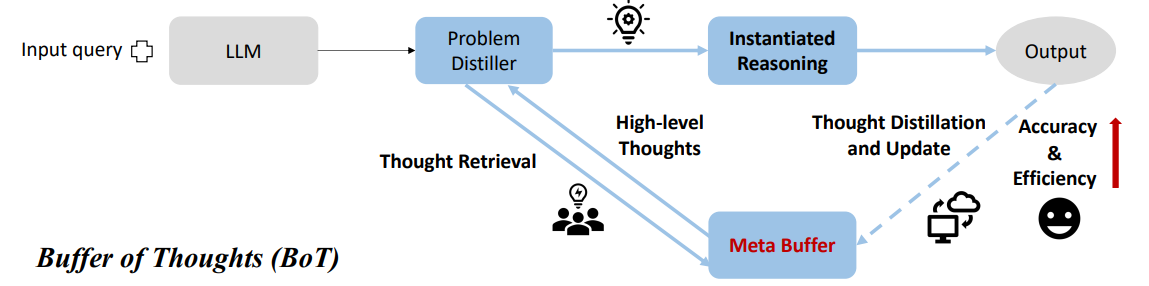
\includegraphics[width=1.0\linewidth]{figure1.png}
  \caption{BoT Framework. Adapted from Figure 1 of the original paper.}
  \label{fig:bot}
\end{figure}

\section{Discussion}
Our project focuses on whether LLMs can play chess through prompting alone, without domain-specific training. The BoT paper inspires a direction for making chess reasoning more general and reusable. Unlike typical CoT prompting, we could maintain a meta-buffer of strategic templates (e.g., fork, pin, center control) and reuse them across similar board states. This approach aligns with BoT’s goal: structured, transferable reasoning that improves over time, even for complex domains like strategic gameplay.


\newpage
\bibliographystyle{plain}
\bibliography{reference}

\end{document}